%%%%%%%%%%%%%%%%% DO NOT CHANGE HERE %%%%%%%%%%%%%%%%%%%% {
    \documentclass[12pt,letterpaper]{article}
    \usepackage{fullpage}
    \usepackage[top=2cm, bottom=4.5cm, left=2.5cm, right=2.5cm]{geometry}
    \usepackage{amsmath,amsthm,amsfonts,amssymb,amscd}
    \usepackage{lastpage}
    \usepackage{enumerate}
    \usepackage{fancyhdr}
    \usepackage{mathrsfs}
    \usepackage{xcolor}
    \usepackage{graphicx}
    \usepackage{listings}
    \usepackage{hyperref}
    \usepackage{float} 
    \usepackage{subfigure}
    \definecolor{codegreen}{rgb}{0,0.6,0}
    \definecolor{codegray}{rgb}{0.5,0.5,0.5}
    \definecolor{codepurple}{rgb}{0.58,0,0.82}
    \definecolor{backcolour}{rgb}{0.95,0.95,0.92}
    
    \lstdefinestyle{mystyle}{
        backgroundcolor=\color{backcolour},   
        commentstyle=\color{codegreen},
        keywordstyle=\color{magenta},
        numberstyle=\tiny\color{codegray},
        stringstyle=\color{codepurple},
        basicstyle=\ttfamily\footnotesize,
        breakatwhitespace=false,         
        breaklines=true,                 
        captionpos=b,                    
        keepspaces=true,                 
        numbers=left,                    
        numbersep=5pt,                  
        showspaces=false,                
        showstringspaces=false,
        showtabs=false,                  
        tabsize=2
    }

    \hypersetup{%
      colorlinks=true,
      linkcolor=blue,
      linkbordercolor={0 0 1}
    }
    
    \setlength{\parindent}{0.0in}
    \setlength{\parskip}{0.05in}
    %%%%%%%%%%%%%%%%%%%%%%%%%%%%%%%%%%%%%%%%%%%%%%%%%%%%%%%%%% }
    
    %%%%%%%%%%%%%%%%%%%%%%%% CHANGE HERE %%%%%%%%%%%%%%%%%%%% {
    \newcommand\course{ECE 271A}
    \newcommand\semester{Fall 2019}
    \newcommand\hwnumber{\#3}                 % <-- ASSIGNMENT #
    \newcommand\NetIDa{Jiaming Lai}           % <-- YOUR NAME
    \newcommand\NetIDb{A53314574}           % <-- STUDENT ID #
    %%%%%%%%%%%%%%%%%%%%%%%%%%%%%%%%%%%%%%%%%%%%%%%%%%%%%%%%%% }
    
    %%%%%%%%%%%%%%%%% DO NOT CHANGE HERE %%%%%%%%%%%%%%%%%%%% {
    \pagestyle{fancyplain}
    \headheight 35pt
    \lhead{\NetIDa}
    \lhead{\NetIDa\\\NetIDb}                 
    \chead{\textbf{\Large Assignment \hwnumber}}
    \rhead{\course \\ \semester}
    \lfoot{}
    \cfoot{}
    \rfoot{\small\thepage}
    \headsep 1.5em
    %%%%%%%%%%%%%%%%%%%%%%%%%%%%%%%%%%%%%%%%%%%%%%%%%%%%%%%%%% }
    
    \begin{document}
     
    \section*{1.Computation Equation}
    % If the Problem is divided into items, use "enumerate"
    Class-conditional:
    \begin{equation}
        P_{x|\mu,\Sigma}=G(x,\mu,\Sigma) \nonumber
    \end{equation}
    where
    \begin{equation}
        \Sigma=\frac{1}{N}\sum_{i=1}^{N}\left(x_i-\frac{1}{N}\sum_{i=1}^{N}
        x_i\right)\left(x_i-\frac{1}{N}\sum_{i=1}^{N}x_i\right)^T \nonumber
    \end{equation}
    Gaussian prior:
    \begin{equation}
        P_{\mu}(\mu)=G(\mu,\mu_0,\Sigma_0) \nonumber
    \end{equation}
    where $\mu_0$ and $\Sigma_0$ is known. The following is the computation equations
    of different classification methods.
    \begin{enumerate}[a)]
        \item 
        predictive distribution:
        \begin{equation}
            P_{x|T}(x|D)=G(x,\mu_n,\Sigma+\Sigma_n) \nonumber
        \end{equation}
        where
        \begin{equation}
            \mu_n=\Sigma_0\left(\Sigma_0+\frac{1}{N}\Sigma\right)^{-1}
            \mu_{ML}+\frac{1}{N}\Sigma\left(\Sigma_0+\frac{1}{N}\Sigma\right)^{-1}
            \mu_0 \nonumber
        \end{equation}
        \begin{equation}
            \Sigma_n=\Sigma_0\left(\Sigma_0+\frac{1}{N}\Sigma\right)^{-1}
            \frac{1}{N}\Sigma \nonumber
        \end{equation}
        \item 
        MAP:
        \begin{equation}
            P_{x|T}(x|D)=G(x,\mu_n,\Sigma) \nonumber
        \end{equation}
        \item 
        ML:
        \begin{equation}
            P_{x|T}(x|D)=G(x,\mu_{ML},\Sigma) \nonumber
        \end{equation}
    \end{enumerate}

    \section*{2.Curves of Classification Error vs $\alpha$}
    % If the Problem is divided into items, use "enumerate"
    \begin{figure}[H]
        \centering 
        \subfigure{
        \label{Fig.D1andS1}
        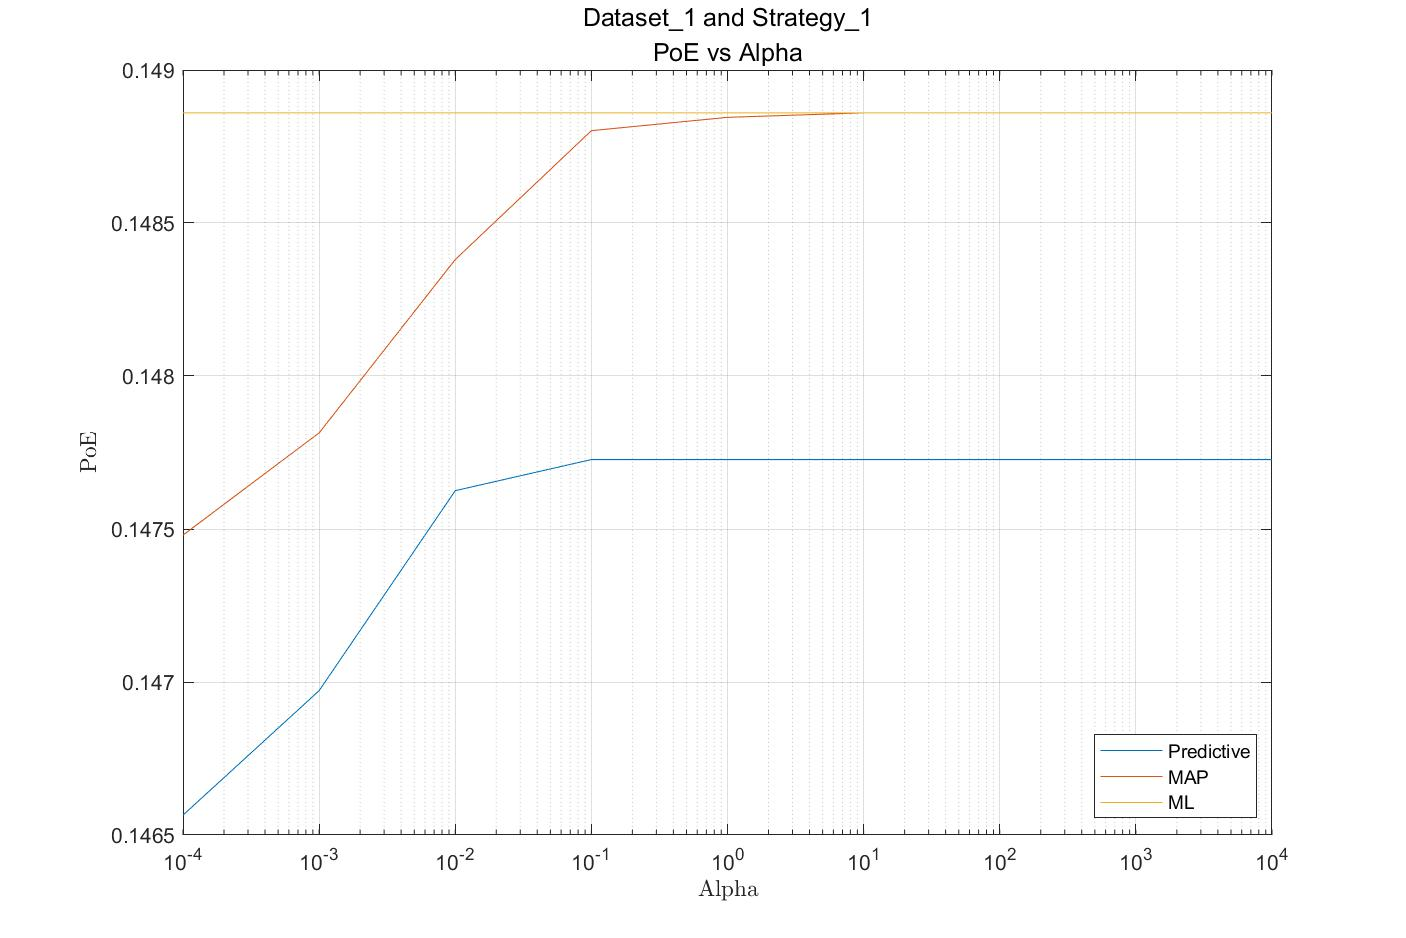
\includegraphics[width=0.45\textwidth]{images/D1andS1.jpg}}
        \subfigure{
        \label{Fig.D1andS2}
        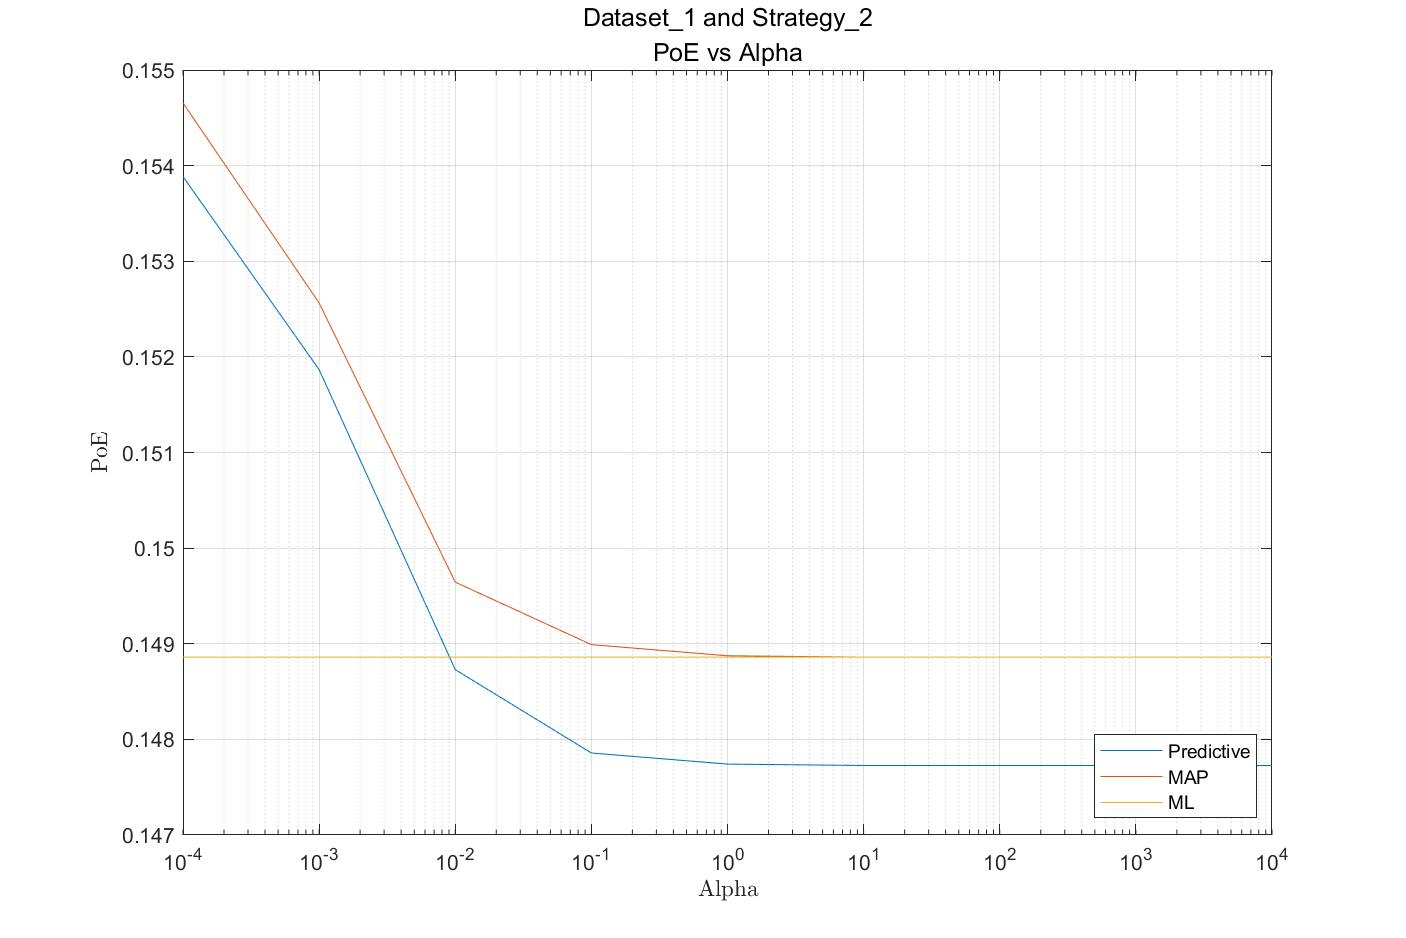
\includegraphics[width=0.45\textwidth]{images/D1andS2.jpg}}
    \end{figure}
    %%%%
    \begin{figure}[H]
        \centering 
        \subfigure{
        \label{Fig.D2andS1}
        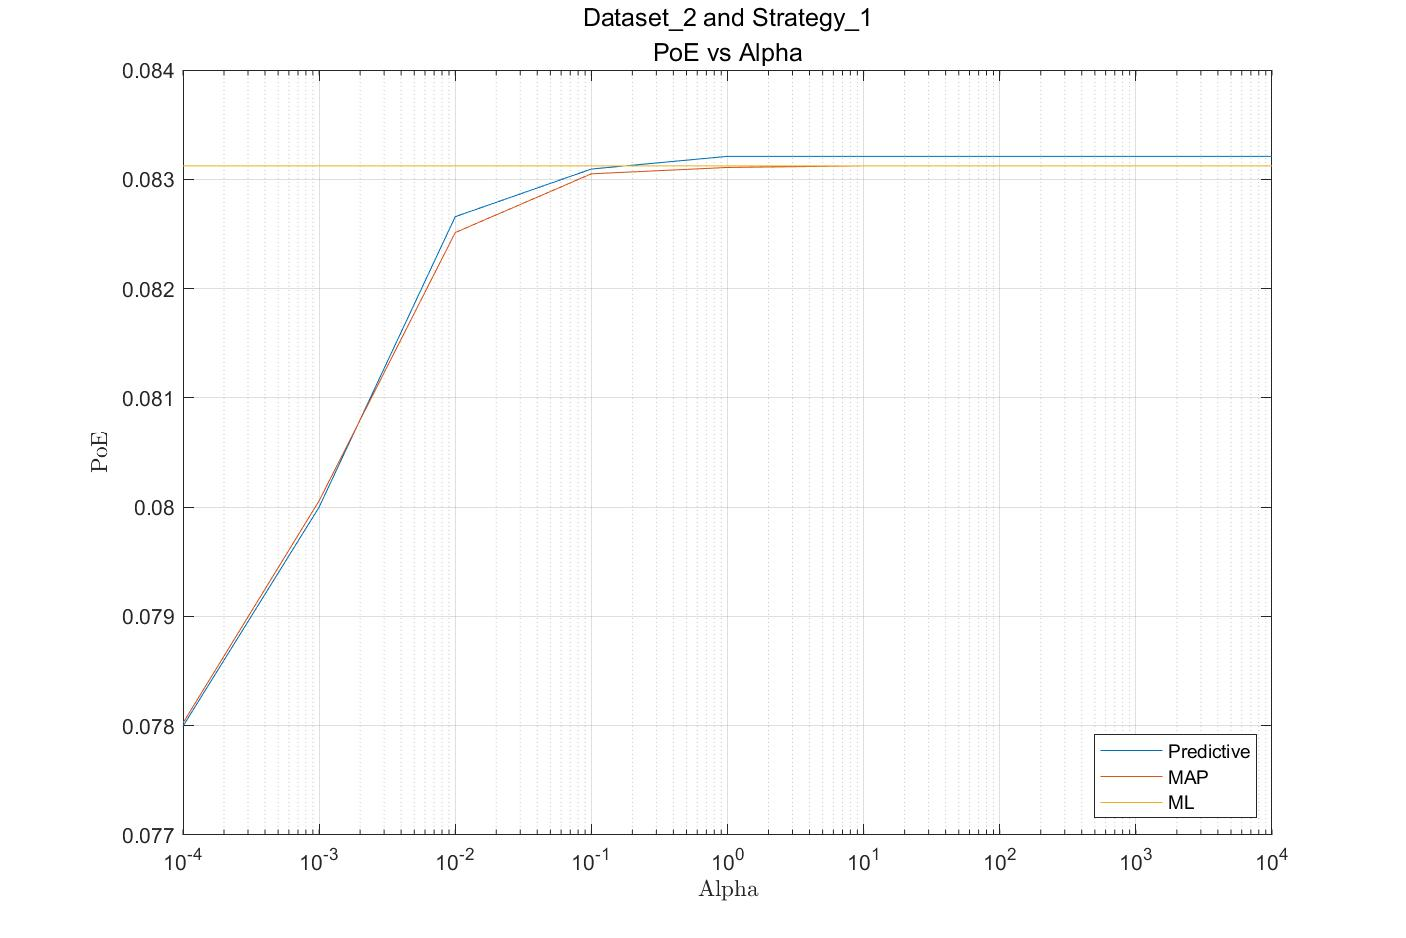
\includegraphics[width=0.45\textwidth]{images/D2andS1.jpg}}
        \subfigure{
        \label{Fig.D2andS2}
        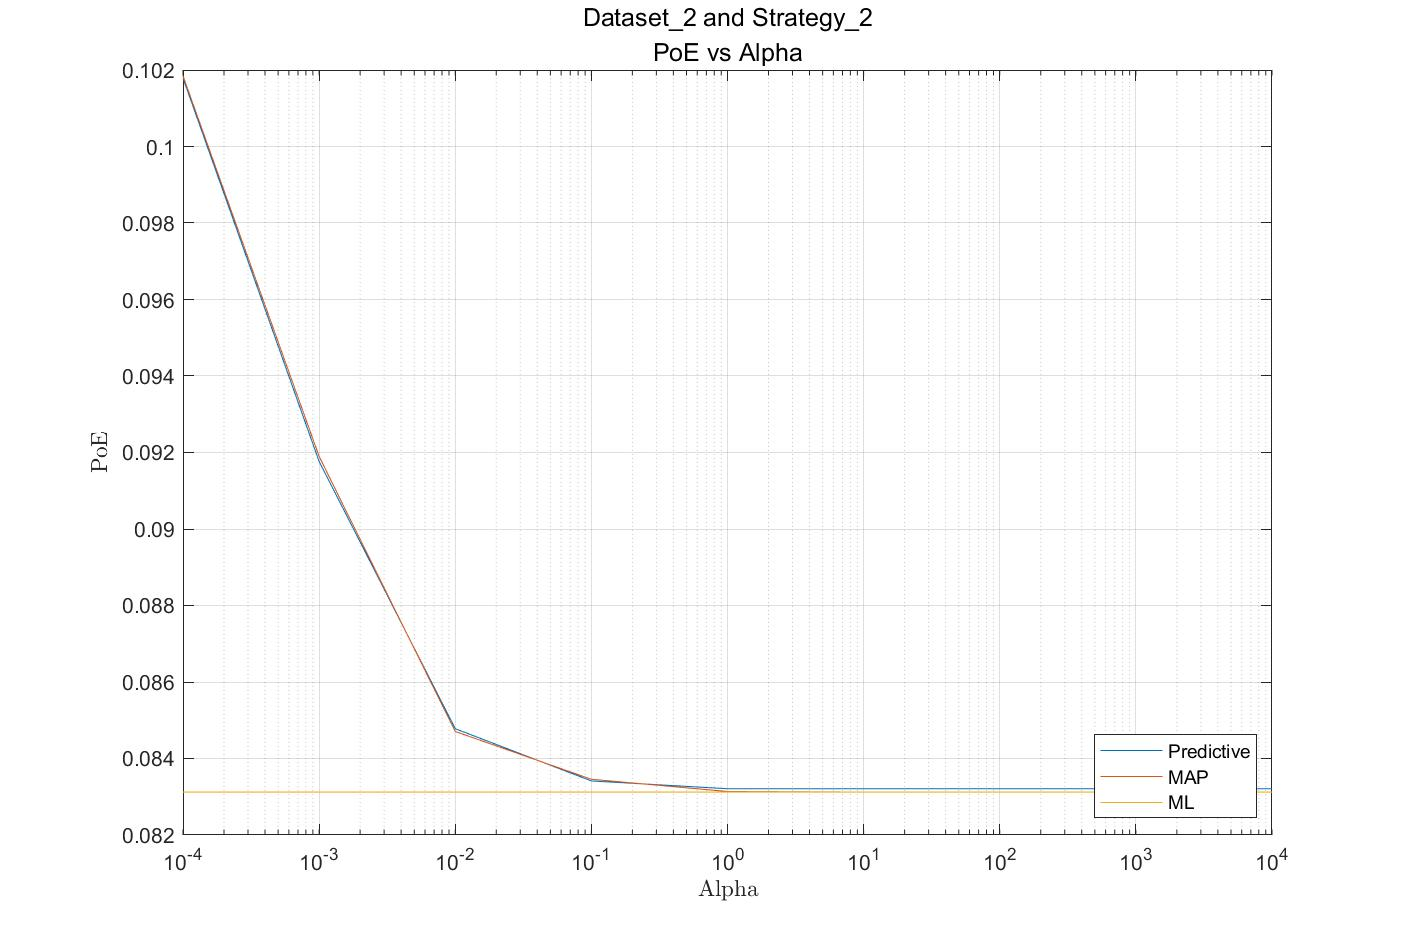
\includegraphics[width=0.45\textwidth]{images/D2andS2.jpg}}
    \end{figure}
    %%%%
    \begin{figure}[H]
        \centering 
        \subfigure{
        \label{Fig.D3andS1}
        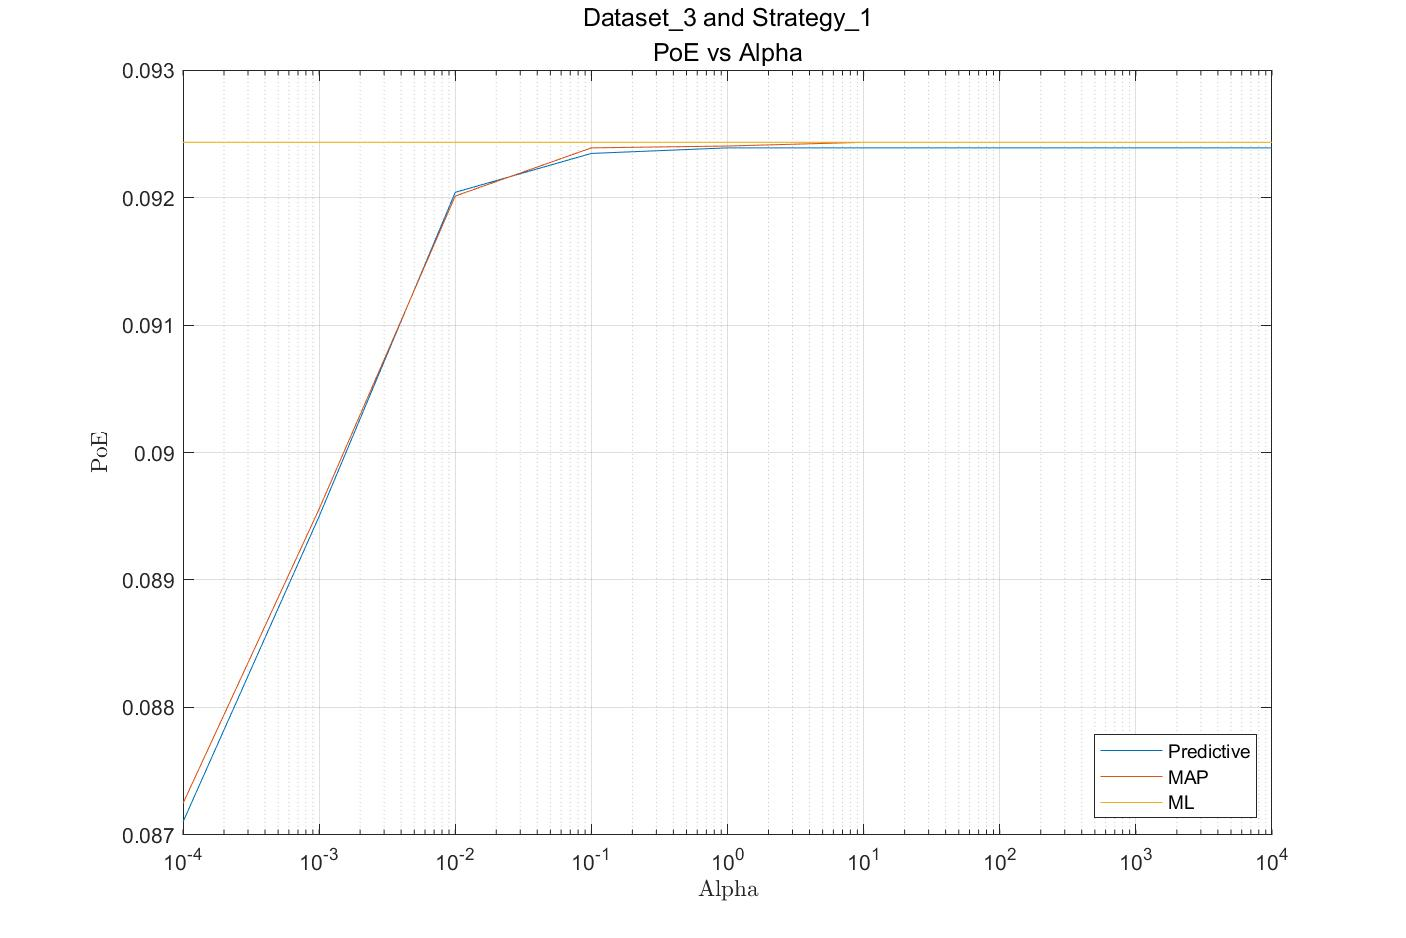
\includegraphics[width=0.45\textwidth]{images/D3andS1.jpg}}
        \subfigure{
        \label{Fig.D3andS2}
        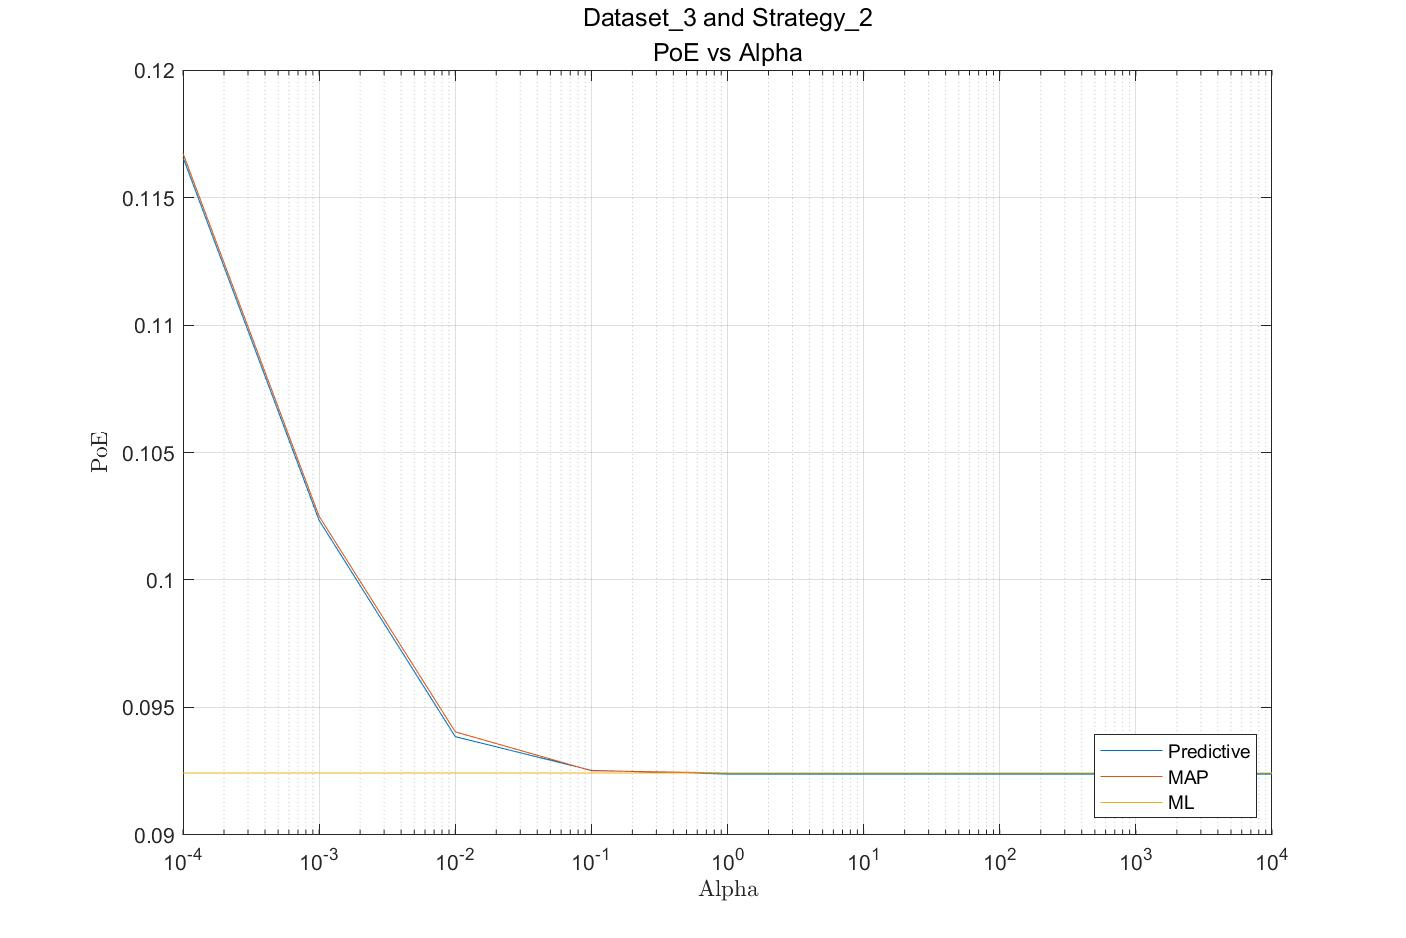
\includegraphics[width=0.45\textwidth]{images/D3andS2.jpg}}
    \end{figure}
    %%%%
    \begin{figure}[H]
        \centering 
        \subfigure{
        \label{Fig.D4andS1}
        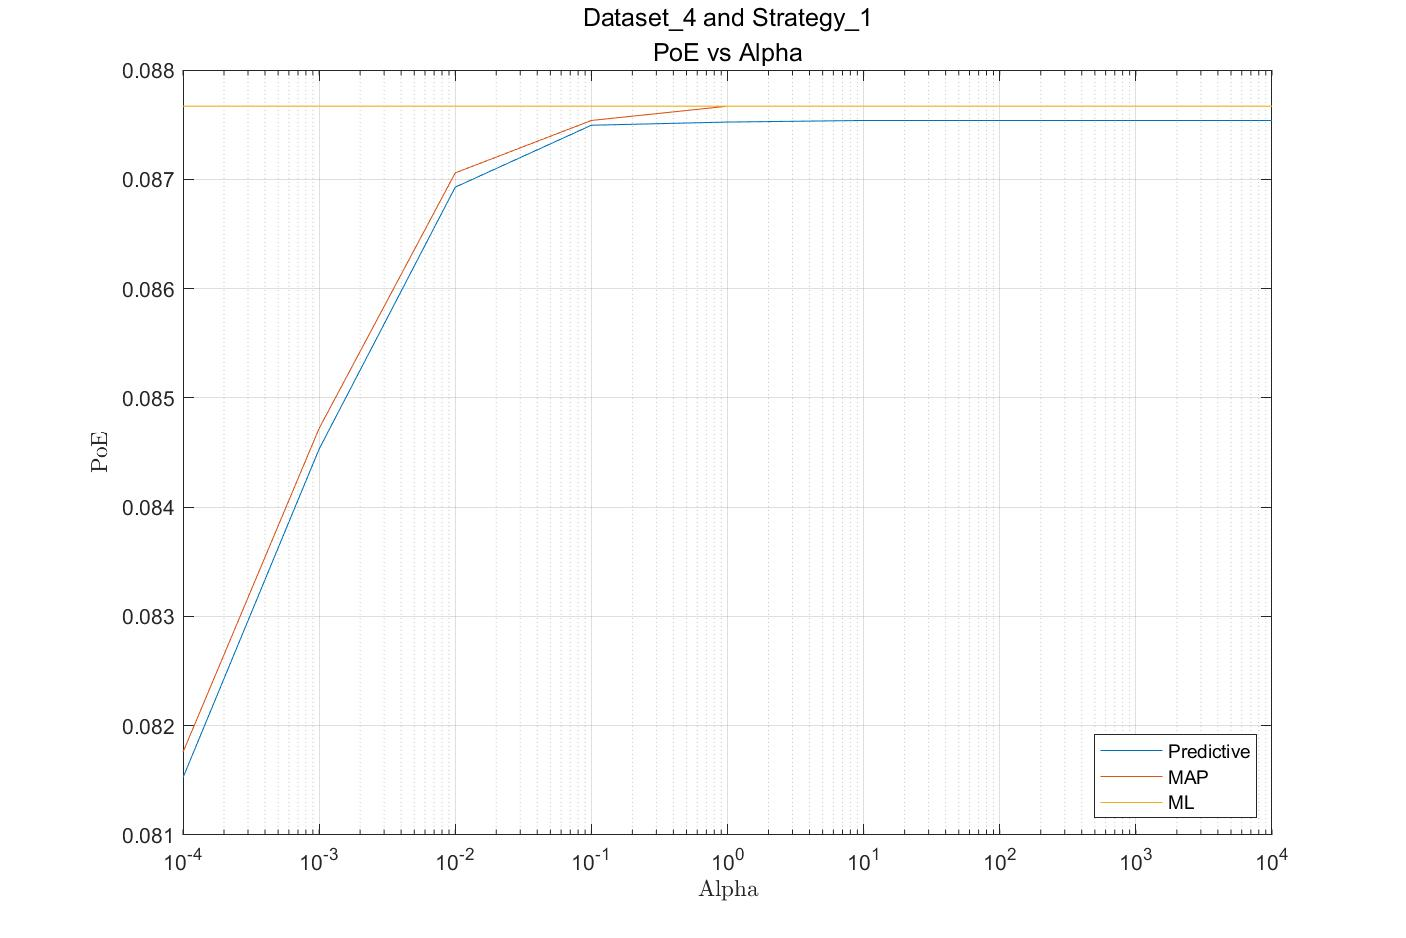
\includegraphics[width=0.45\textwidth]{images/D4andS1.jpg}}
        \subfigure{
        \label{Fig.D4andS2}
        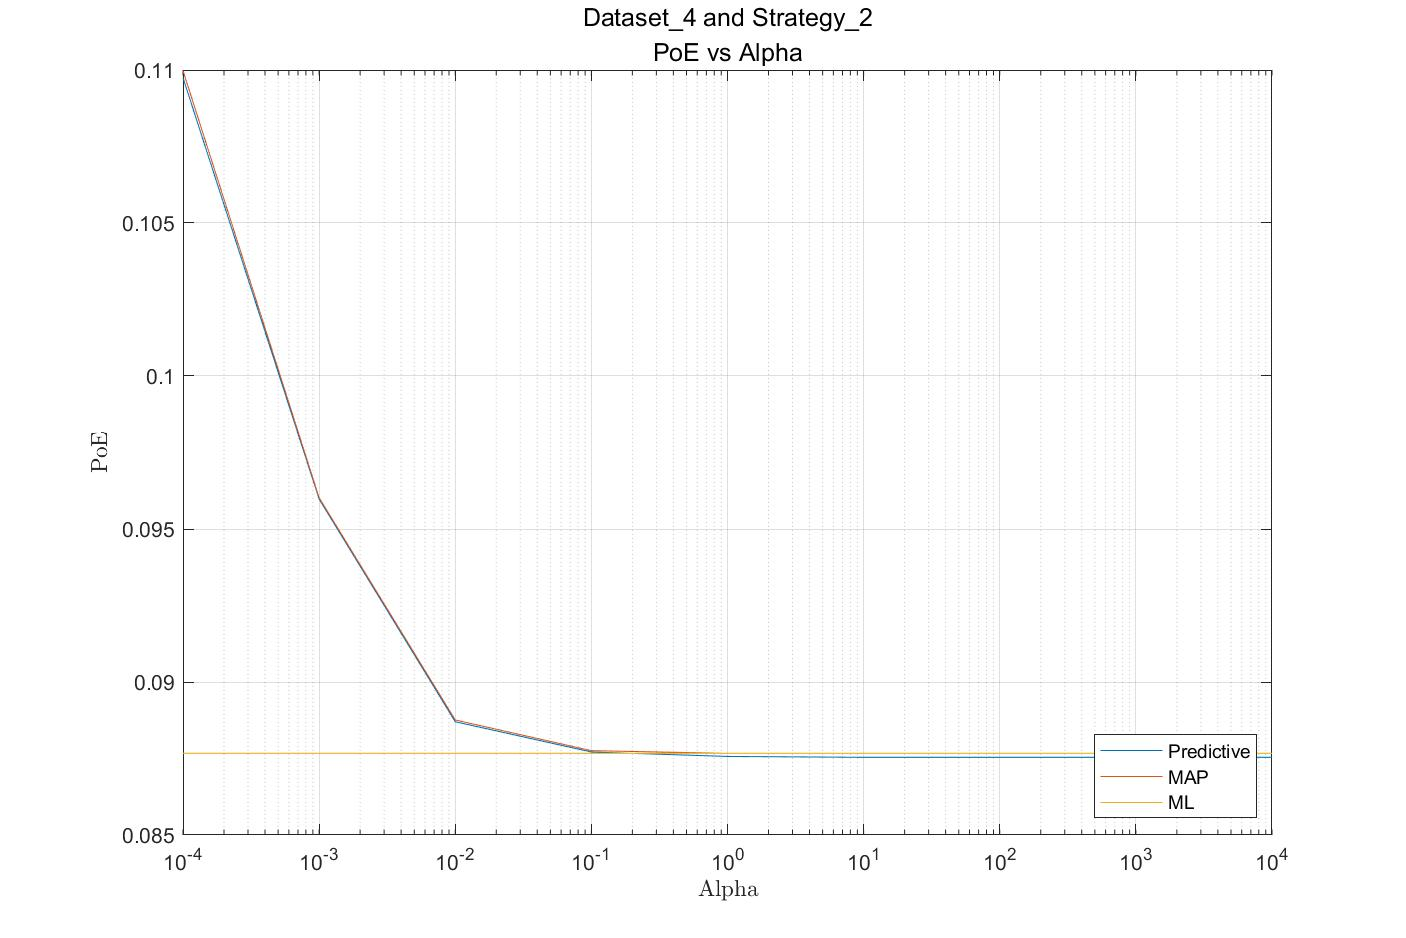
\includegraphics[width=0.45\textwidth]{images/D4andS2.jpg}}
    \end{figure}

    \section*{3.Observation and Explaination}
    \begin{enumerate}[a)]
        \item 
        The relative behavior of these three curves.\\
        Observation: in strategy 1, the ML line is a constant (horizontal) line.
        The PoE corresponding to MAP solution increases as alpha increases, and finally
        converges to ML line. The PoE corresponding to predictive solution increases as alpha increases,
        and finally goes to a constant value. This constant value is obviously smaller than ML in
        dataset1, a little bit bigger than ML in dataset2 and a little bit smaller than ML in dataset3\&4.
        In strategy 2, things would be different, but we will discuss in section (c).\\

        Explaination: ML line is a constant (horizontal) line because ML method has nothing to do with
        alpha. As alpha increases, the prior information becomes more uncertain, making the PoE of MAP
        and predictive solution increases. For the MAP solution, increase of alpha would push $\mu_n$ more
        and more closet to $\mu_{ML}$, and finally let the MAP solution and ML solution nearly the same when
        alpha is large enough. For the predictive solution, increase of alpha would also push $\mu_n$ more
        and more closet to $\mu_{ML}$. Meanwhile, $\Sigma_n$ would approximate to $\frac{1}{N}\Sigma$, leading
        $\Sigma+\Sigma_n$ approximate to $\Sigma+\frac{1}{N}\Sigma$. Hence predictive solution would go
        to a constant value when alpha is large enough. This constant value varies depending on sample number
        in different dataset. That is why we can see the constant values in dataset1,2,3\&4 are different.
        \item 
        How that behavior changes from dataset to dataset.\\
        Observation: the PoE corresponding to predictive solution is obviously smaller than MAP solution in
        dataset1. However, in dataset2,3\&4, PoE of predictive solution and MAP solution are nearly the same.
        In dataset2, predictive solution performs a little worse than MAP solution. But in dataset3\&4, 
        predictive solution performs a little better than MAP solution.

        Explaination: when sample number of dataset (for example, dataset1) is relatively small, then predictive solution
        use more information of prior, leading predictive solution performs better than MAP solution
        and ML solution. However, when sample number is relatively large (for example, dataset2,3\&4),
        $\Sigma+\Sigma_n$ would approximate to $\Sigma$, making predictive solution performs nearly similiar
        with MAP solution. However, when the alpha is large enough, they will converge to constant value,
        as discuss in section (a). The final PoE differ depending on sample number but the difference is small
        because at this time, the impact of alpha is predominant.
        \item 
        How all of the above change when strategy 1 is replaced by strategy 2?\\
        Observation: In strategy 2, at a small alpha, PoE of predictive solution and MAP solution are
        obviously worse than ML solution. As alpha increases, PoE of predictive solution and MAP solution
        would decrease. As for MAP solution, it would again converges to ML line when alpha is large enough.
        The reason is the same as we discuss in section(a). As for predictive solution, in dataset1, predictive
        solution performs obviously better than MAP solution. The final constant PoE is also obviously better
        than MAP and ML solution. But in dataset2,3\&4, performance of predictive solution is nealy similiar
        with MAP solution. The reason is the same as we discuss in section (b).

        Explaination: The difference between strategy 1 and strategy 2 is the mean of first DCT coefficients.
        We plot the marginal distribution of first DCT coefficience in Homework2 and already find the obvious
        difference of mean between background and foreground. Hence strategy 2 actually provides a bad prior information
        and play a bad guide. Predictive solution and MAP solution use information from prior, so in strategy 2,
        when alpha is relatively small, PoE of predictive solution and MAP solution is obvious large than ML solution.
        But when alpha increases, the prior becomes less important and ML estimation becomes predominant. Hence MAP solution
        would converges to ML line, and predictive solution would go to constant value.
    \end{enumerate}

    \section*{Appendix}
    The following is the Matlab code.

    \subsection{HW3\_solution.m}
    \lstset{style=mystyle}
    \lstinputlisting[language=Matlab]{HW3_solution.m}

    \subsection{fun\_general.m}
    This function receives parameters: train data, array of alpha and strategy we want to choose,
    and compute error using MAP-BDR, Bayes-BDR and ML-BDR.
    \lstset{style=mystyle}
    \lstinputlisting[language=Octave]{myfunction/fun_general.m}

    \subsection{fun\_bayesBDR.m}
    This function performs Bayes-BDR.
    \lstset{style=mystyle}
    \lstinputlisting[language=Octave]{myfunction/fun_bayesBDR.m}

    \subsection{fun\_mapBDR.m}
    This function performs MAP-BDR.
    \lstset{style=mystyle}
    \lstinputlisting[language=Octave]{myfunction/fun_mapBDR.m}

    \subsection{fun\_mlBDR.m}
    This function performs ML-BDR.
    \lstset{style=mystyle}
    \lstinputlisting[language=Octave]{myfunction/fun_mlBDR.m}

    \subsection{fun\_zigzag.m}
    This function compute DCT coefficients and save it as DCT\_coefficience.mat.
    \lstset{style=mystyle}
    \lstinputlisting[language=Octave]{myfunction/fun_zigzag.m}

    \subsection{fun\_mvgaussian.m}
    This function perfroms multi-gaussian.
    \lstset{style=mystyle}
    \lstinputlisting[language=Octave]{myfunction/fun_mvgaussian.m}

    \subsection{fun\_cov.m}
    \lstset{style=mystyle}
    \lstinputlisting[language=Octave]{myfunction/fun_cov.m}

    \subsection{fun\_mean.m}
    \lstset{style=mystyle}
    \lstinputlisting[language=Octave]{myfunction/fun_mean.m}

    \end{document}